\documentclass[12pt,twoside]{article}
\usepackage{amsmath, amssymb}
\usepackage{amsmath}
\usepackage{fancyhdr,parskip}
\usepackage[active]{srcltx}
\usepackage{amssymb}
\usepackage{amscd}
\usepackage{makeidx}
\usepackage{amsthm}
\usepackage{algorithm}
\usepackage{algpseudocode}
\usepackage{fancyhdr}
\usepackage{graphics}
\usepackage{amsmath, amssymb}
\usepackage{amsmath}
\usepackage[active]{srcltx}
\usepackage{amssymb}
\usepackage{amscd}
\usepackage{makeidx}
\usepackage[dvips]{graphicx}
\usepackage{longtable}
\usepackage{tabularx}
\usepackage[table,xcdraw]{xcolor}
\usepackage{color}
\usepackage[hidelinks]{hyperref}
\usepackage[backend=biber,style=apa]{biblatex}
\usepackage{longtable}
\usepackage{tabularx}
\usepackage[table,xcdraw]{xcolor}
\usepackage{color}
\usepackage[hidelinks]{hyperref}
\usepackage{multirow}
\usepackage{algorithm}
\usepackage{algpseudocode}

\usepackage[ruled,vlined]{algorithm2e}
\include{pythonlisting}
\usepackage{fancyhdr,graphicx,amsmath,amssymb}
\renewcommand{\algorithmicrequire}{\textbf{Input:}}
\renewcommand{\algorithmicensure}{\textbf{Output:}}
\renewcommand{\tablename}{Tabla}
\renewcommand{\figurename}{Figura}
\renewcommand{\baselinestretch}{1}
\setcounter{page}{1}
\setlength{\textheight}{21.6cm}
\setlength{\textwidth}{14cm}
\setlength{\oddsidemargin}{1cm}
\setlength{\evensidemargin}{1cm}
\pagestyle{myheadings}
\thispagestyle{empty}
\markboth{\small{Pr\'actica 4. Luis Francisco Renteria Cedillo, Denzel Omar Vazquez Perez.}}{\small{.}}
\date{}
\begin{document}
    \begin{figure}[h]
    \vspace{-3cm} \hspace{-2cm} \setlength{\unitlength}{1mm}
    \begin{picture}(15,25)(-10,0)
    
\includegraphics[width=16.5cm,height=2.8cm]{imagenes/titulo.png}
    \end{picture}
    \end{figure}
    \vspace{0cm}
    \centerline{\bf An\'alisis de Algoritmos, Sem: 2022-2, 3CV11, Pr\'actica 4, 11 de mayo de 2022}
    \centerline{}
    \begin{center}
    \Large{\textsc{Pr\'actica 4: Divide y vencer\'as}}
    \end{center}
    \centerline{}
    \centerline{\bf {Luis Francisco Renteria Cedillo, Denzel Omar Vazquez Perez.}}
    \centerline{}
    \centerline{$lrenteriac1400@alumno.ipn.mx, dvazquezp1600@alumno.ipn.mx$}
    \newtheorem{Theorem}{\quad Theorem}[section]
    \newtheorem{Definition}[Theorem]{\quad Definition}
    \newtheorem{Corollary}[Theorem]{\quad Corollary}
    \newtheorem{Lemma}[Theorem]{\quad Lemma}
    \newtheorem{Example}[Theorem]{\quad Example}
    \bigskip
    \textbf{Resumen:} En el presente documento se muestra la implementaci\'on y el an\'alisis tanto {\it a Priori} como {\it a Posteriori} de dos algoritmos, cuyo objetivo de ambos es girar una imagen textual en arte ASCII 90° utilizando estrategias de dise\~no de algoritmos como {\it "Divide y Vencer\'as"} y {\it "Fuerza Bruta"}.

    {\bf Palabras Clave:} Imagen, Rotar, An\'alisis,  Recursividad, Fuerza bruta. 
    
    \section{Introducci\'on}
    Con el tiempo el uso de algoritmos ha aumentado teniendo un crecimiento exponencial puesto a la mejora de estrategias para dar soluci\'on a cualquier problema de programaci\'on, ya que estos tienen una suma importancia en el desarrollo de cualquier aplicaci\'on.\\
    \\
    Ante esto, el llevar a cabo un an\'alisis de complejidad del algoritmo permite conocer si este es adecuado para el caso presentado, dada su entrada de datos de tama\~no n, pero ¿qu\'e es n?, la definici\'on de n depende de la naturaleza del problema, ya que puede representar el tama\~no de una arreglo, los nodos de un grafo o el n\'umero de elementos de una matriz.\\
    Como ejemplo de lo dicho anteriormente son la im\'agenes digitales, que al contener caracter\'isticas discretas, se puede asociar a una matriz de tama\~no $MxN$ donde cada elemento de esta guarda su definici\'on de color al tomar valores n\'umericos de 0 a 255.\\
    \\
    As\'i al conocer lo antes mencionado es posible las operaciones como de ajuste de brillo, invertir colores, el ajuste de canales y la rotaci\'on de la imagen misma, pero ¿c\'omo se logran a cada una de estas?.\\
    \\
    De este modo en el presente documento se implementan 2 algoritmos para rotaci\'on de matrices que permitir\'an girar 90° una imagen textual en arte ASCII, haciendo uso de la estrategia {\it "Divide y vencer\'as"} comparando esta misma ante la implementaci\'on iterativa del problema a resolver.

    \section{Conceptos te\'oricos}
        \subsection{Imagen}
        Una imagen es una funci\'on bidimensional $f(x,y)$, cuyo valor representa la intensidad de la imagen en las coordenadas $(x,y)$.
        \begin{figure}[h]
            \centering
            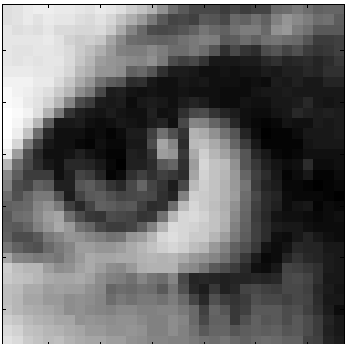
\includegraphics[height=5cm]{imagenes/con1.png}
            \caption{Imagen digital}
        \end{figure}
        \subsection{Imagen textual en arte ASCII}
        Las im\'agenes textuales en arte ASCII son la formaci\'on de figuras o "arte" a partir de los caracteres disponibles en el gr\'afico conocido como ASCII . Estas im\'agenes eran populares antes de Internet y la banda ancha cuando los usuarios se conectaban a través de un BBS (Bulletin Board System) el cual era una pequeña red donde los usuarios se comunicaban y compartían cosas.
        
        \subsection{Recursividad}
        Es una opci\'on distinta para llevar a cabo construcciones de repetici\'on (ciclos). Se puede utilizar en toda situaci\'on en la cual la soluci\'on logre ser expresada como una serie de movimientos, pasos o transformaciones gobernadas por un grupo de normas no ambiguas.
        
        \subsection{Fuerza bruta}
        Es un enfoque de soluci\'on, usualmente basado en el enunciado del problema y las definiciones de conceptos involucrados.
        \subsection{Divide y vencer\'as}
        Algunos algoritmos se orientan a la hora de resolver un problema utilizando el enfoque conocido como "divide y vencerás" donde la cuestión a tratar se divide en distintos subproblemas parecidos al problema raíz, pero más pequeños, estos se resuelven recursivamente, es decir, una y otra vez, y después las soluciones a estos se juntan para dar una solución final al problema principal.
        El modelo se lleva a cabo en tres pasos por cada grado de recursividad que pasa:
       \begin{itemize}
        \item "Dividir" la cuestión a tratar en diversos subproblemas siendo estos más pequeños que el problema principal.
        \item "Vencer" los subproblemas dándoles solución de manera recursiva. Hay que tener en cuenta que, si el subproblema es muy pequeño, simplemente se resuelve directamente sin hacer ninguna recursividad.
        \item "Combina" las soluciones obtenidas de los subproblemas anteriores en la solución del problema raíz.
        \end{itemize}
        
        \subsection{Algoritmos}
         El siguiente algoritmo tiene la funcionalidad de rotar una imagen 90° utilizando la estrategia de divide y vencerás. Como puede observarse, siempre se trabaja con cuadrantes, y cada uno de ellos se divide a su vez a nuevas matrices hasta llegar a las submatrices 2x2. En ese instante se rotan los elementos y regresa dicha submatriz al proceso recursivo que a su vez rota los cuadrantes relacionados hasta llegar a la función original.
        
        \begin{algorithm}[H]
\SetAlgoLined
\textbf{Input: }{Matriz $\textbf{i}$, tamaño de matriz $\textbf{n}$}\;\\
\KwResult{Imagen rotada 90° }
\textbf{Rotar}{($i,n$)}\\

  \eIf{n==2}{
   \Return [i[0][1] i[1][1] , i[0][0] i[1][0]]\;
   }{
    t = Matriz(n,n)\; \\
    t.segundoCuadrante = rotar(primerCuadrante(i),n/2)\;\\
    t.tercerCuadrante = rotar(segundoCuadrante(i),n/2)\;\\
    t.primerCuadrante = rotar(cuartoCuadrante(i),n/2)\;\\
    t.cuartoCuadrante = rotar(tercerCuadrante(i),n/2)\;
    
    \Return t\;
  }
 
 \caption{Rotar Divide y Venceras}
\end{algorithm}

El algoritmo que se presenta a continuación, convierte cada una de las columnas originales de la imagen en columnas para crear la nueva imagen rotada. Dicho proceso se le conoce como fuerza bruta, ya que cada uno de los elementos de la fila le corresponde un elemento de la columna de la imagen original. Esto se logra con la función Transpuesta que de antemano se sabe que tiene complejidad lineal.
\begin{algorithm}[H]

\textbf{Input: }{Matriz $\textbf{m}$, tamaño de matriz $\textbf{n}$}\;\\
\KwResult{Imagen rotada 90° }
\textbf{Rotar}{($i,n$)}\\
    t = Matriz(n,n)\;\\
    \For {i=0 to n} 
        {t.fila(n-i) = Transpuesta(m.columna(i)}\\
    \EndFor
 
 \caption{Rotar por fuerza bruta}
\end{algorithm}


    \newpage
    \section{Experimentaci\'on y resultados}
    El problema a resolver es el implementar una función que rote 90° una imagen de entrada con formato bmp, dicha imagen debe tener dimensiones de potencia de 2 tanto en alto como en ancho.
    \subsection{Funci\'on implementada por medio de la estrategia Divide y Vencer\'as}
        \subsubsection{An\'alisis a Priori}
        Se determina que el tama\~no del problema esta definido por el tama\~no de los lados de la matriz a dividir, dado que ambos lados son iguales, entonces se tiene que $n=2^{k}$ por tanto al dividir a la mitad a $n$ se tiene que $\frac{n}{2}=2^{k-1}$, v\'ease Figura 2.
        \begin{figure}[H]
        \centering
        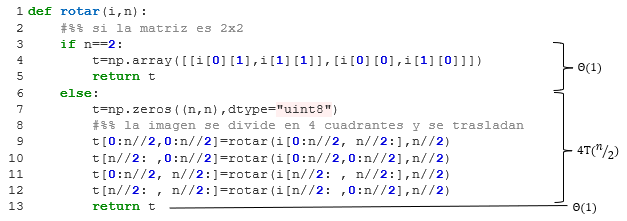
\includegraphics[height=5.5cm]{imagenes/c1.png}
        \caption{Análisis por bloques de código de la función rotar().}
        \end{figure}
        As\'i en la Figura 2 se muestra la implementaci\'on de la estrategia Divide y vencer\'as para la rotaci\'on de la matriz, donde para cada bloque de c\'odigo se muestra la obtenci\'on del orden de complejidad para el peor caso de este por medio del análisis a bloques del código, por lo que se determina que la funci\'on de recurrencia de este algoritmo es 
        $$T(n)= \left\{ \begin{array}{lcc}
            \Theta(1) &   si  & n=2 \\
            \\ 4T(\frac{n}{2})+\Theta(1) &  si & n>2
            \end{array}
            \right.$$
        Sea $a=4$, $b=2$ y $f(n)=\Theta(1)=C$ donde $a\geq1$ y $b>1$ se tiene que
        $$n^{\log_b{a}}=n^{\log_2{4}}=n^{2}$$
        por otro lado se tiene que
        $$f(n)=C\in\mathcal{O}(n^{\log_2{4}-\epsilon})=\mathcal{O}(n^{2-2})$$
        Entonces por el Teorema Maestro, caso I)
        $$T(n)=\Theta(n^{\log_b{a}})=\Theta(n^{2})$$
        \subsubsection{An\'alisis a Posteriori}
        
        Para el análisis a posteriori se realizo una gráfica de ejecuciones vs n, dado que la imagen tiene dimensiones n*n, v\'ase Figura 3.
        \\
        As\'i siguiendo la definición formal de $\Theta(n)$, y proponiendo los valores de: $C_{1}=20$, $C_{2}=40$ y $n_{0}=64$ puesto que se tiene una gráfica de una ecuación cuadrática. Dichos valores obedecen a la desigualdad de la definición formal de $\Theta(n)$ ya que se acotan los puntos tanto en la forma superior como inferior, además se cumplen a partir del punto de cruce propuesto. 
        Por lo tanto la complejidad del algoritmo según el análisis a posteriori es de $\Theta(n^2)$.
        \\
        \begin{figure}[H]
        \centering
        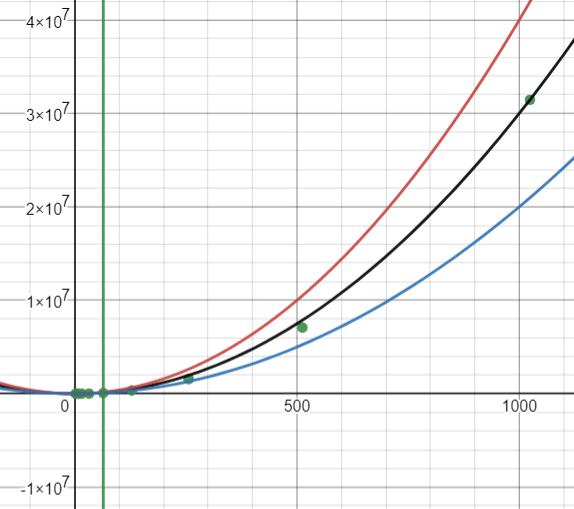
\includegraphics[width=8cm]{imagenes/g1.png}
        \caption{Gráfico de ejecuciones vs n para el algoritmo 1}
        \end{figure}
        
    \subsection{Funci\'on implementada por medio de fuerza bruta}
        \subsubsection{An\'alisis a Priori}
        En la siguiente figura observamos que el análisis por bloques del código nos indica que la función transpose convierte una fila en columna, dicha función tiene una complejidad de O(n), y dado que está en un ciclo for que se repite n veces, entonces esta tiene una complejidad de O($n^2$).
        
        Podemos observar que python puede manejar matrices con índices negativos, esto sucede porque se le aplica la función modulo a los índices negativos regresando valores validos, facilitando nuestra función de rotación.
        \\
        \begin{figure}[H]
        \centering
        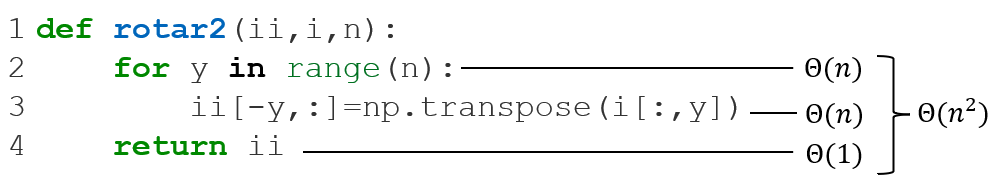
\includegraphics[height=2.0cm]{imagenes/c2.png}
        \caption{Análisis por bloques de código de la función rotar().}
        \end{figure}
        
        \subsubsection{An\'alisis a Posteriori}
        Para el desarrollo del análisis a posteriori realizamos una gráfica de ejecuciones vs n, dado que nuestra imagen tiene dimensiones n*n. A continuación se presenta la gráfica de dichos puntos.
        \\
        \begin{figure}[h]
        \centering
        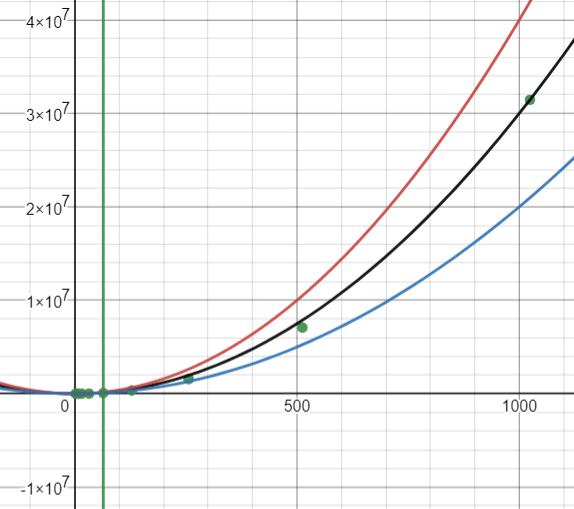
\includegraphics[height=7cm]{imagenes/g1.png}
        \caption{Gráfico de ejecuciones vs n para el algoritmo 2}
        \end{figure}
        
        Siguiendo la definición formal de $\Theta(n)$ proponemos los valores de: $C_{1}=2$, $C_{2}=4$ y $n_{0}=64$ puesto que se tiene una gráfica de una ecuación cuadrática. Dichos valores obedecen a la desigualdad de la definición formal de $\Theta(n)$ ya que se acotan los puntos tanto en la forma superior como inferior, además se cumplen a partir del punto de cruce propuesto. Por lo tanto la complejidad del algoritmo según el análisis a posteriori es de $\Theta(n^2)$
        En la siguiente figura se muestran los resultados al rotar la imagen 90° tanto para el algoritmo 1 como el 2.
        \\
        \begin{figure}[h]
        \centering
        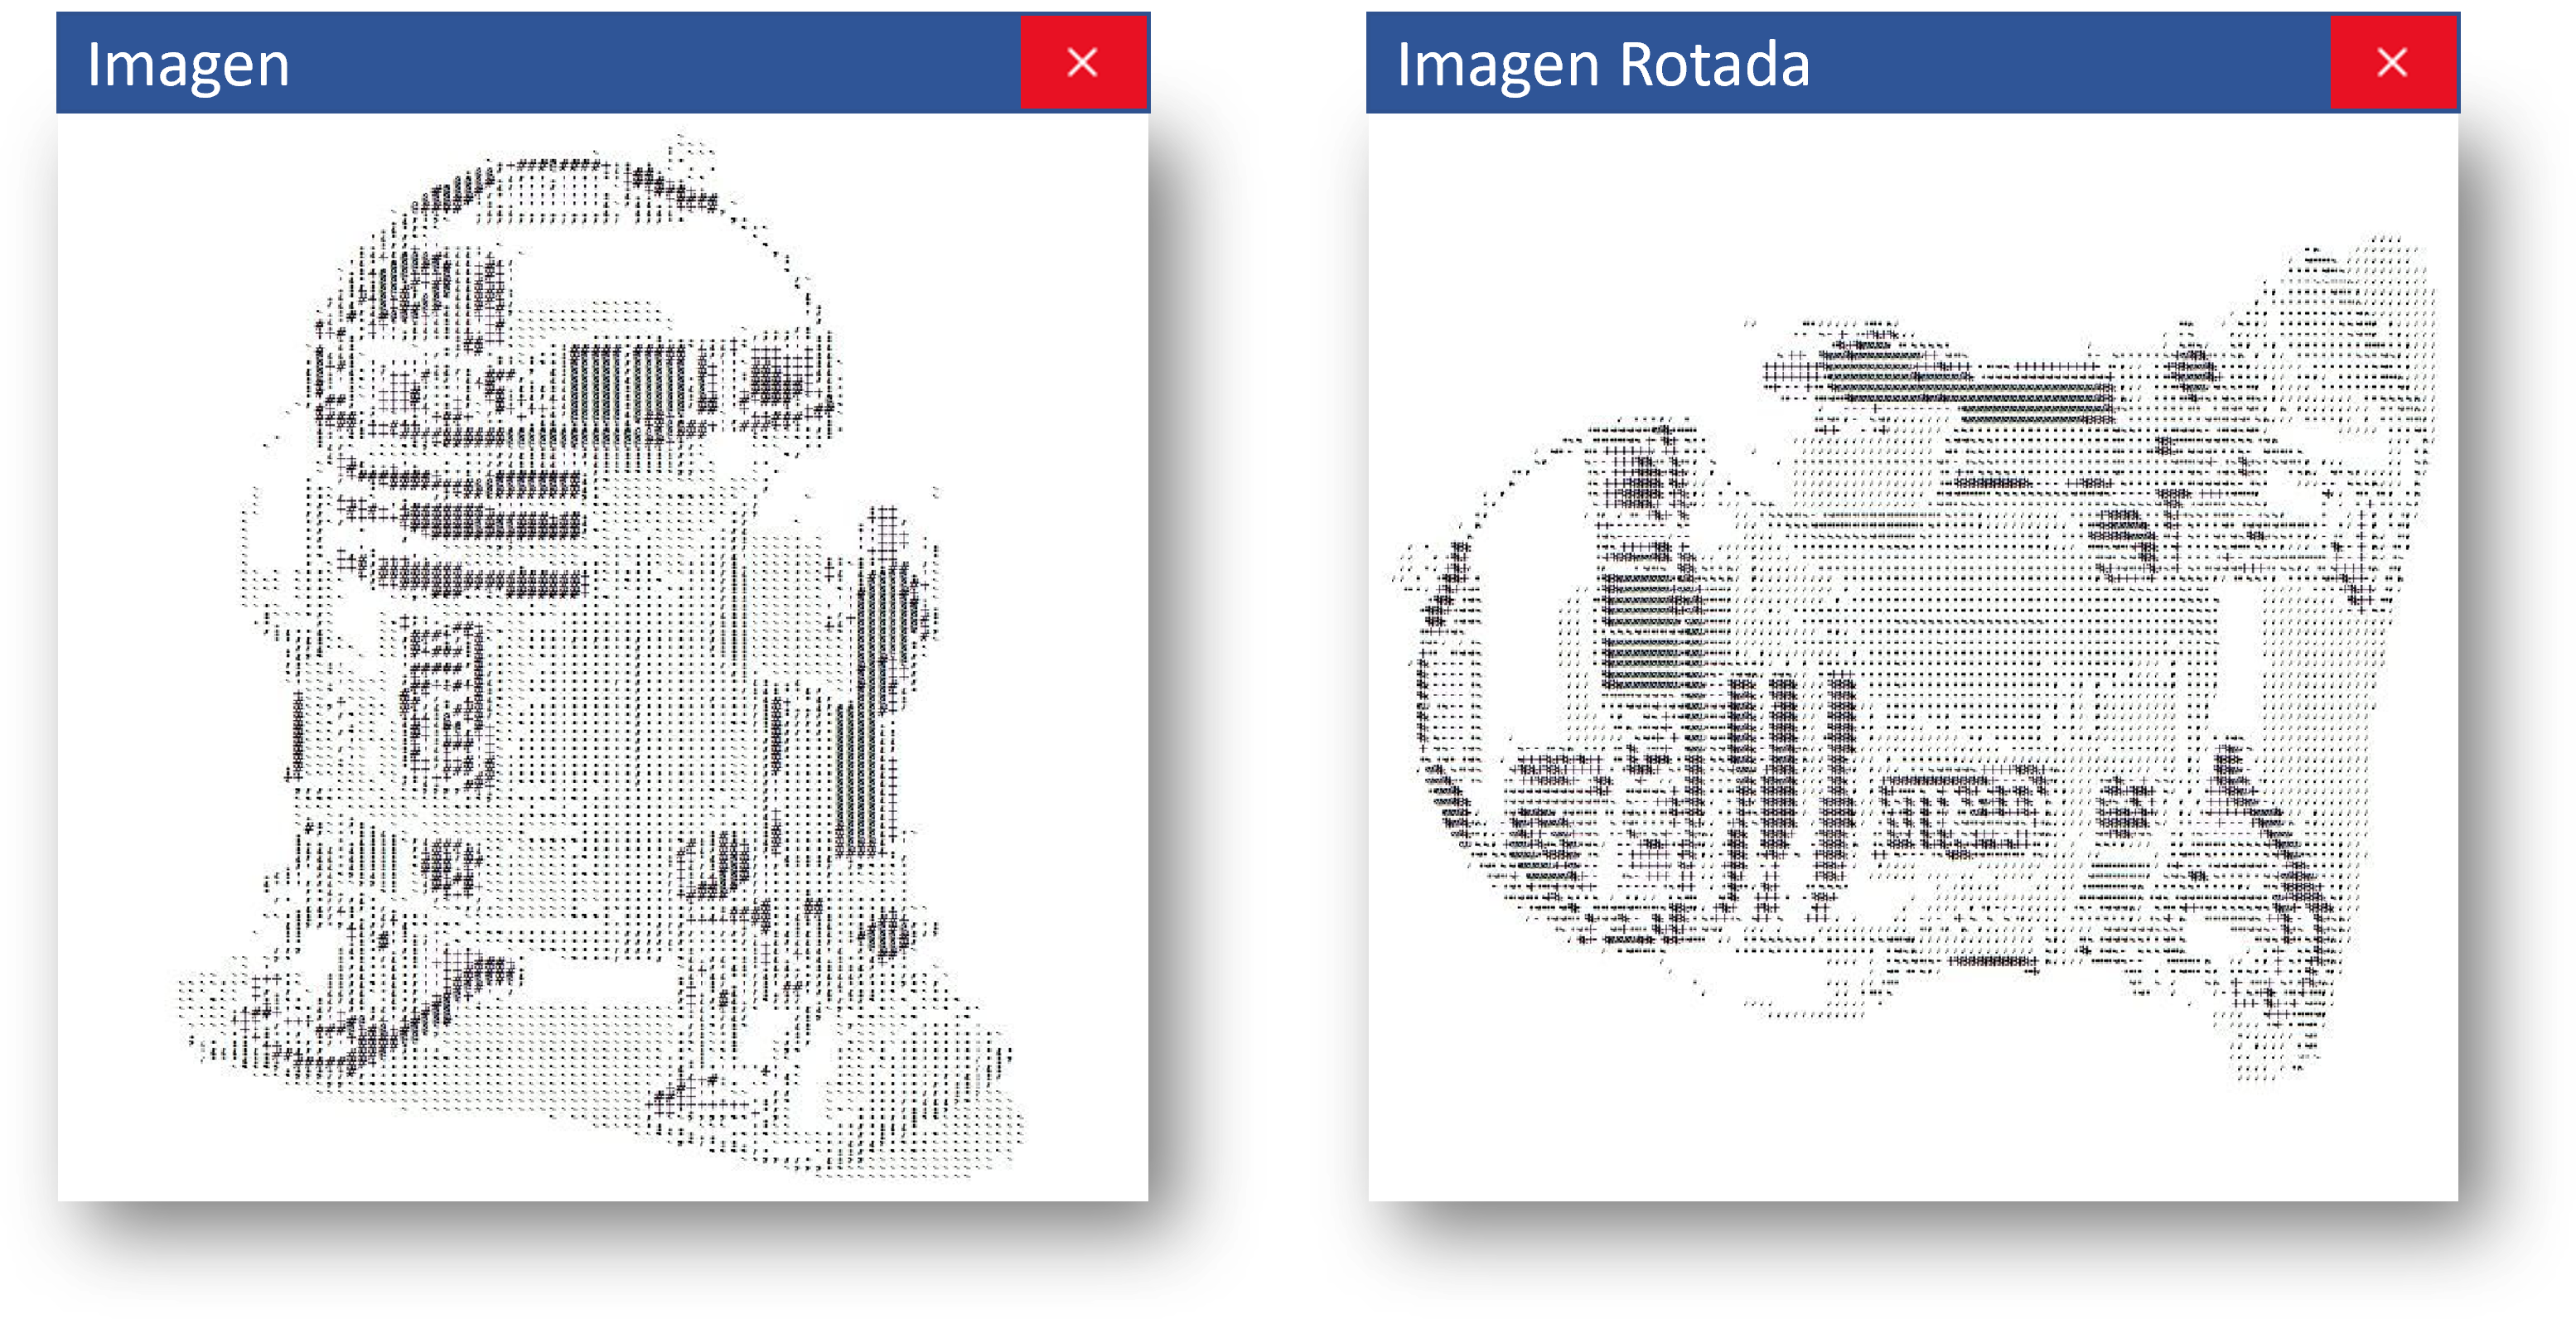
\includegraphics[width=14cm]{imagenes/r1.png}
        \caption{Resultado al rotar la imagen}
        \end{figure}
        
    \newpage
    \section{Conclusiones}
    \textbf{\large Luis Francisco Renteria Cedillo}
    \begin{figure}[H]
        \centering
        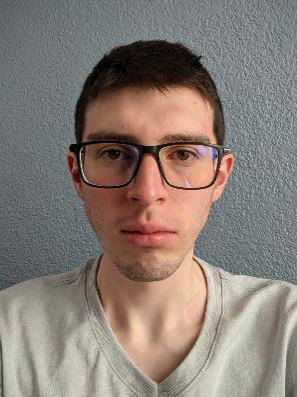
\includegraphics[angle=0, scale=0.5]{imagenes/foto1.png}
    \end{figure}
     Siguiendo el lema de "Dividir, vencer y combinar" logramos realizar esta practica y comprender mejor el funcionamiento dicha estrategia, ya que es fácil reconocer en todo momento como la imagen es dividida recursivamente en cuatro cuadrantes hasta que la matriz llega a tamaño 2x2. una vez llegado a este punto se rotan los valores y regresa al bloque anterior, a partir de aquí los valores son ahora submatrices de tamaño n*n, y se realiza la misma operación hasta combinar tanto los cuadrantes como los canales RGB que componen la imagen.
        
    A pesar de que en la experimentación nos arrojaron resultados que indican que se tiene la misma complejidad tanto algoritmo 1 como el 2, se logra un mayor comprendimiento de como funcionan ambas estrategias.
    
    \newpage
    \textbf{\large Denzel Omar Vazquez Perez}
        \begin{figure}[H]
            \centering
            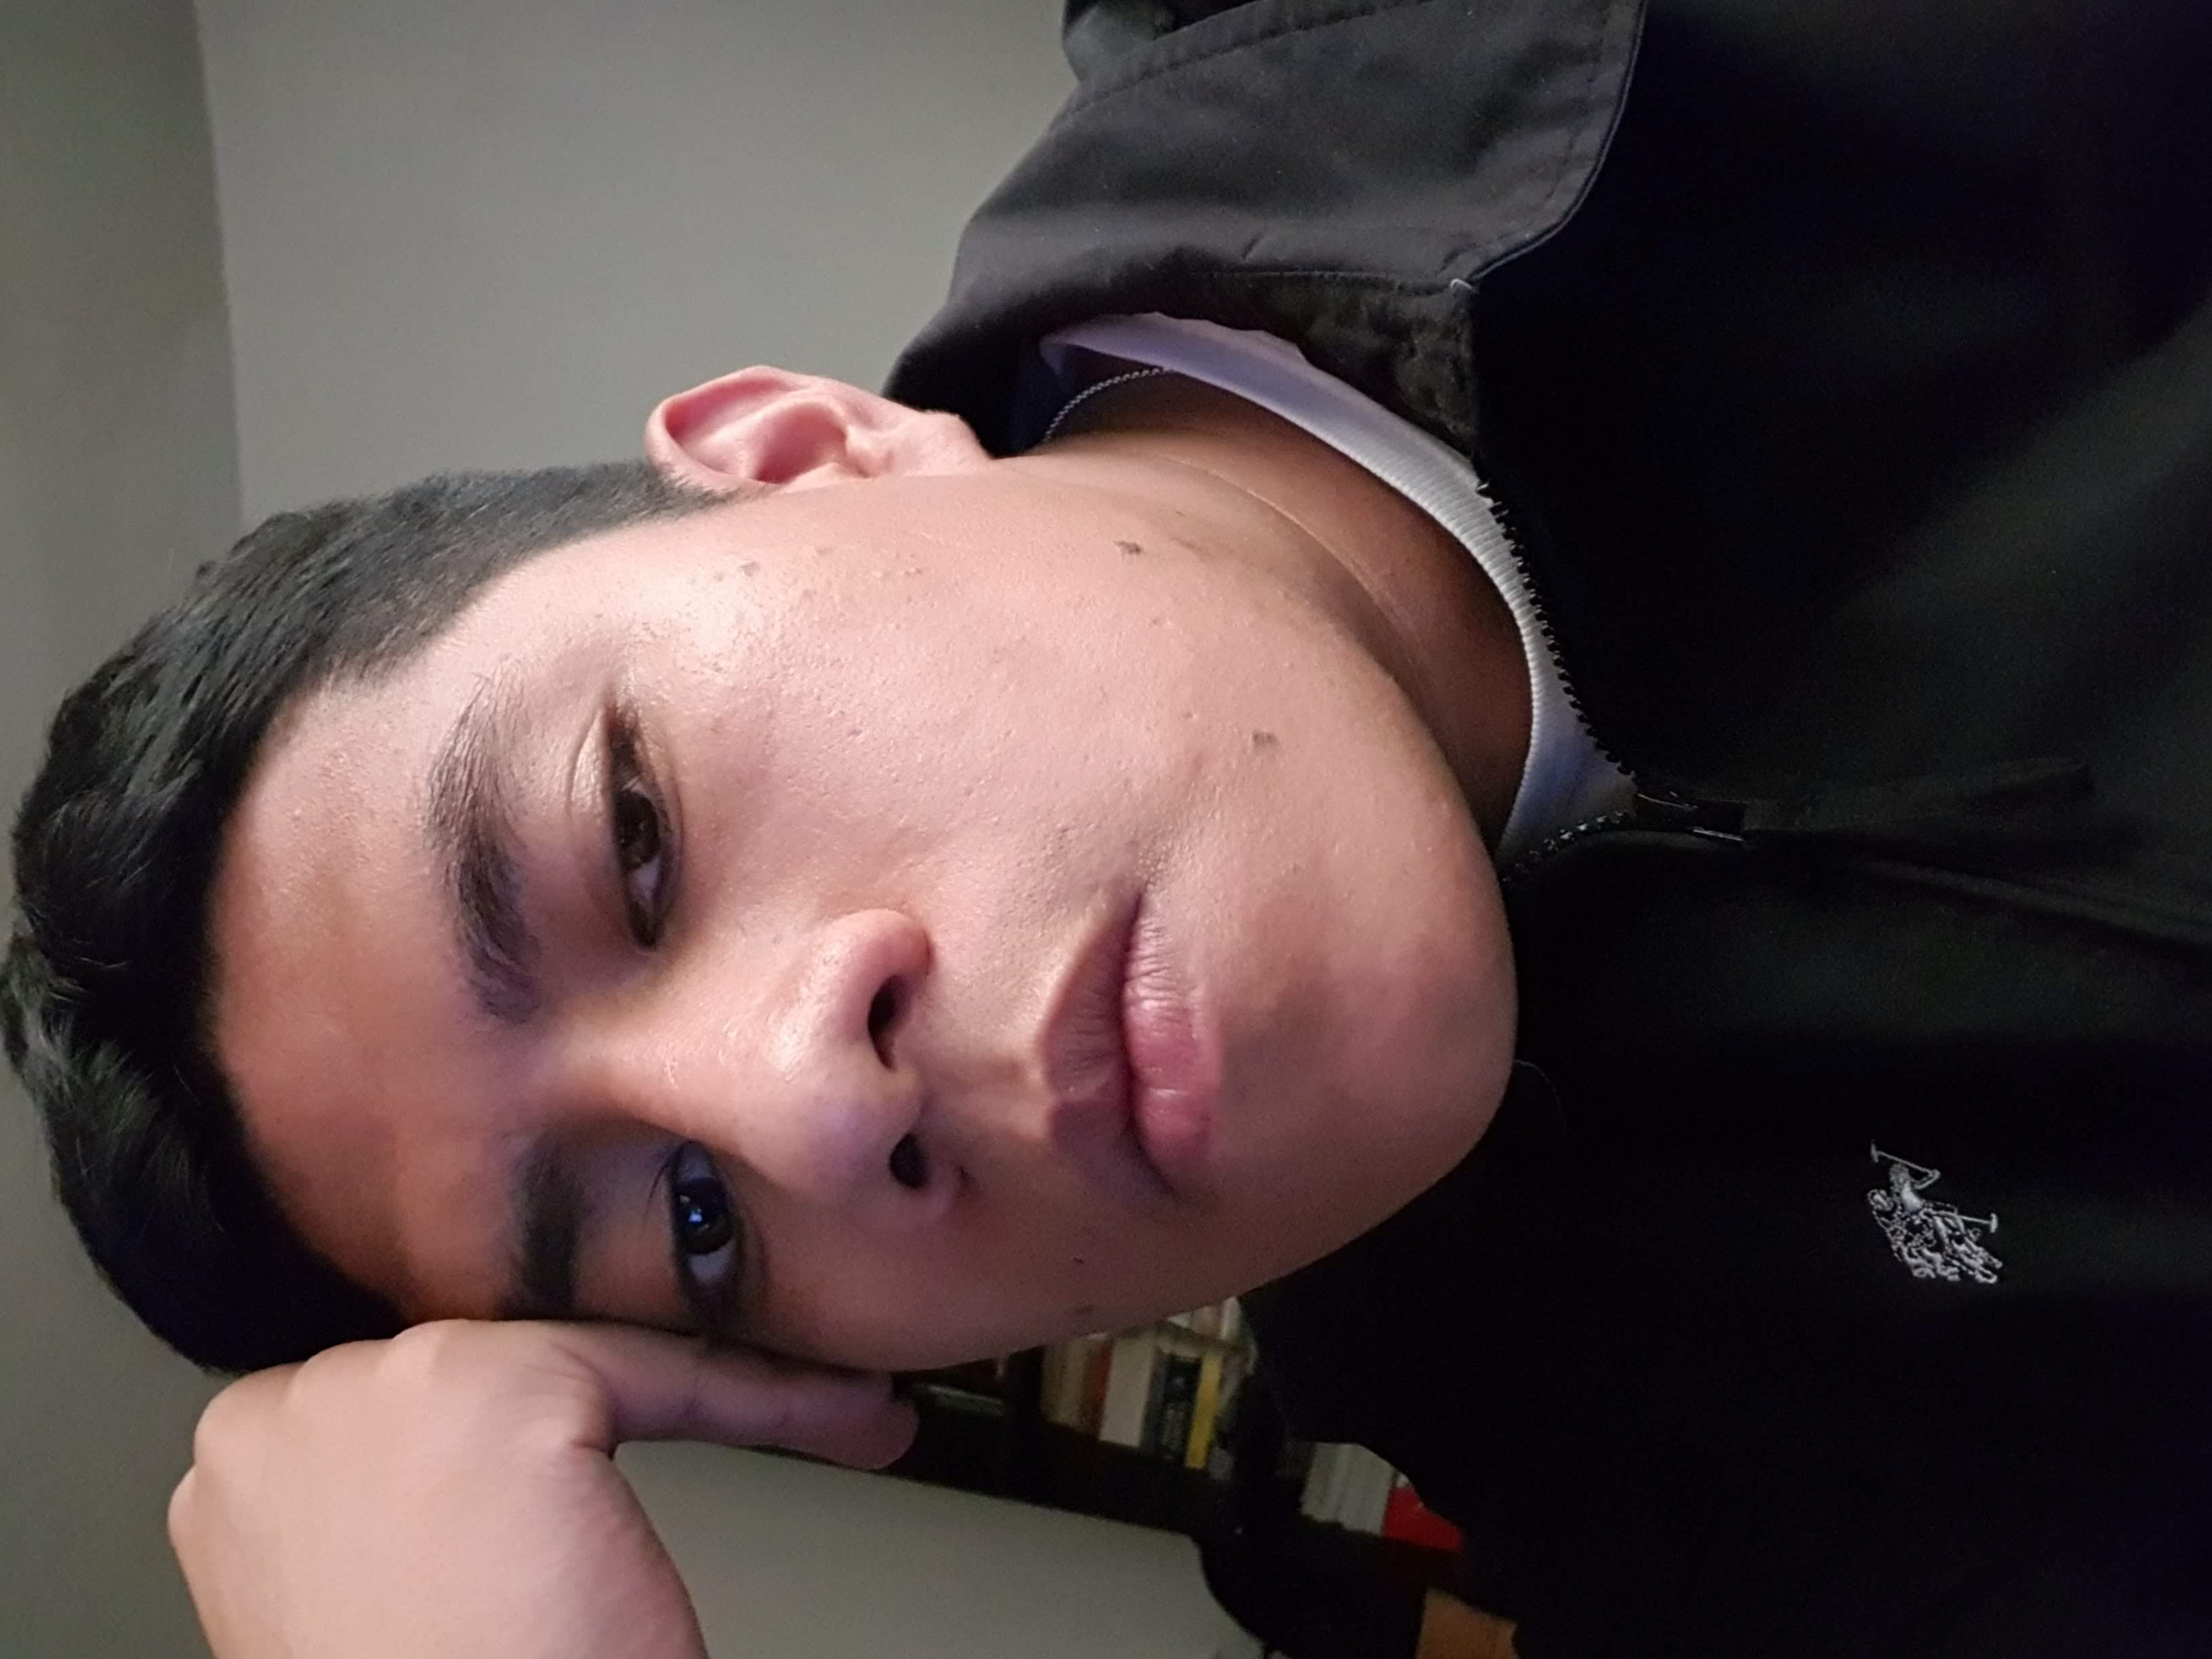
\includegraphics[angle=-90, scale= 0.05]{imagenes/foto2.jpg}
        \end{figure}
        Es importante percatarse que la utilizaci\'on de la estrategia {\it "Divide y vencer\'as"} permite tener ventajas sobre cualquier otro tipo enfoque de soluci\'on, la separaci\'on en subproblemas ayuda a que el manejo de datos o del tama\~no del problema sea digerible y se pueda lograr obtener buenos resultados a partir de la divisi\'on de tareas y recursividad de estas.\\
        \\
        Esto se logra observar en los resultados y experimentaci\'on de la pr\'actica para rotar cada una de las matrices por las que se conforma la imagen, algo interesante es que pude ver que el algoritmo implementado con {\it "Divide y vencer\'as"} puede que no tenga ninguna ventaja ante el de fuerza bruta.\\
        \\
        Sin embargo su complejidad espacial disminuye al no hacer uso de una matriz auxiliar dando soluci\'on al problema de forma paralela, teniendo mayor eficiencia frente a cualquier algoritmo cl\'asico de rotaci\'on de matrices.
    \newpage
    \section{Anexo}
    \subsection{Probar por sustituci\'on hacia atr\'as que \texorpdfstring{$T(n)\in\theta(n\log_2{(n)})$}{Lg} dado que \texorpdfstring{$T(n)$}{Lg} esta definido por la ecuaci\'on de recursividad: }
        $$T(n)= \left\{ \begin{array}{lcc}
            \Theta(1) &   si  & n=1 \\
            \\ 2T(\frac{n}{2})+Cn &  si & n>1
            \end{array}
            \right.$$
        \textbf{Sol.}\\
        Sea $n=2^{k}~\Rightarrow~k=\log_2{(n)}$ se tiene que $$T(2^{k})= \left\{ \begin{array}{lcc}
                        \Theta(1) &   si  & k=0\\
                        \\ 2T(2^{k-1})+C2^{k} &  si & k>0
                        \end{array}
                \right.$$\\
        Resolviendo por sustituci\'on hacia atr\'as se tiene\\
        \begin{align}
            T(2^{k})&=2T(2^{k-1})+C2^{k}\nonumber\\
            &=2[2T(2^{k-2})+C2^{k-1}]+C2^{k}\nonumber\\
            &=4T(2^{k-2})+2C2^{k-1}+C2^{k}\nonumber\\
            &=4[2T(2^{k-3})+C2^{k-2}]+2C2^{k-1}+C2^{k}\nonumber\\
            &=8T(2^{k-3})+4C2^{k-2}+2C2^{k-1}+C2^{k}\nonumber\\
            &=8[2T(2^{k-4})+C2^{k-3}]+4C2^{k-2}+2C2^{k-1}+C2^{k}\nonumber\\
            &=16T(2^{k-4})+8C2^{k-3}+4C2^{k-2}+2C2^{k-1}+C2^{k}\nonumber\\
            &\vdots\nonumber\\
            (i)&=2^{i}T(2^{k-i})+2^{i-1}C2^{k-i+1}+\cdots+C2^{k}\nonumber\\
            & para~K=i \Rightarrow K-i=0\nonumber\\
            &=2^{k}T(2^{0})+2^{k-1}C2+\cdots+C2^{k}\nonumber\\
            &=2^{k}T(1)+2^{k-1}C2+\cdots+C2^{k}\nonumber\\
            &=2^{k}[C+2^{-1}C2+\cdots+C]\nonumber\\
            & donde~2^{-1}C2+\cdots+C = C\sum_{j=1}^{k}\frac{2^{j}}{2^{j}}=C\sum_{j=1}^{k}{1}=Ck\therefore\nonumber\\
        \end{align}
        \begin{align}
            &=2^{k}[C+Ck]\nonumber\\
            &=C2^{k}+Ck2^{k}\nonumber\\
            &Sustituyendo~n=2^{k}~\Rightarrow~k=\log_2{(n)}\nonumber\\
            &=Cn+Cn\log_2{(n)}=C[n+n\log_2{(n)}]\nonumber\\
            &\therefore T(n)\in \Theta(n\log_2{(n)})\nonumber
        \end{align}
    \subsection{Utilizando decremento por uno pruebe que \texorpdfstring{$T(n)\in\mathcal{O}(n^{2})$}{Lg} donde \texorpdfstring{$T(n)$}{Lg} es la ecuaci\'on de recursividad:}
    $$T(n)=T(n-1)+C(n+1)$$
    \textbf{Sol.}\\
    Resolviendo por decremento por uno se tiene que:
    $$f(n)=C(n+1)$$
    luego sabiendo que el orden de complejidad esta determinado por la siguiente expresi\'on se tiene que
    \begin{align}
            T(n)&=\sum_{j=1}^{n}{f(j)}\nonumber\\
            &=\sum_{j=1}^{n}{f(j+1)}\nonumber\\
            &=\sum_{j=1}^{n}{C(j+1)}=\sum_{j=1}^{n}{Cj+C1}\nonumber\\
            & \textit{despu\'es} \nonumber\\
            &= {C}\sum_{j=1}^{n}{j}+ {C}\sum_{j=1}^{n}{1}\nonumber\\
            &= C\frac{n(n+1)}{2}+Cn = C\frac{n^{2}+n}{2}+Cn\nonumber\\
            &\therefore T(n)\in \mathcal{O}(n^{2})\nonumber
    \end{align}
    \newpage
    \subsection{Utilizando Teorema Maestro pruebe que \texorpdfstring{$T(n)\in\Omega(n\log_2{(n)})$}{Lg} donde \texorpdfstring{$T(n)$}{Lg} es la ecuaci\'on de recursividad:}
    $$T(n)=2T(\frac{n}{2})+\Theta(n)$$
    \textbf{Sol.}\\
    Sea $a=2$, $b=2$ y $f(n)=\Theta(n)=Cn$ donde $a\geq1$ y $b>1$ se tiene que
    $$n^{\log_b{a}}=n^{\log_2{2}}=n$$
    por otro lado se tiene que
    $$f(n)=Cn\in\Theta(n^{\log_2{2}})=\Theta(n)$$
    Entonces por el Teorema Maestro, caso II)
    $$T(n)=\Theta(n^{\log_b{a}} \log_2{n})=\Theta(n\log_2{n})$$
    Finalmente, $T(n)\in\Theta(n\log_2{n})$ ssi $T(n)\in\mathcal{O}(n\log_2{n})$ y $T(n)\in\Omega(n\log_2{n})$.
    
    \subsection{Comprobar que la multiplicaci\'on usual tiene complejidad \texorpdfstring{$\Theta(n^{2})$}{Lg}}
    \textbf{Sol.}\\
    Se propone la funci\'on multiplication la cual permite manejar la longitud o cifra de n\'umeros como un arreglo, a continuaci\'on se muestra el an\'alisis por bloques de c\'odigo que determina que la complejidad del algoritmo $T(n)\in\Theta(n^{2})$ ante este problema, v\'ease la Figura 7.
    \begin{figure}[h]
        \centering
        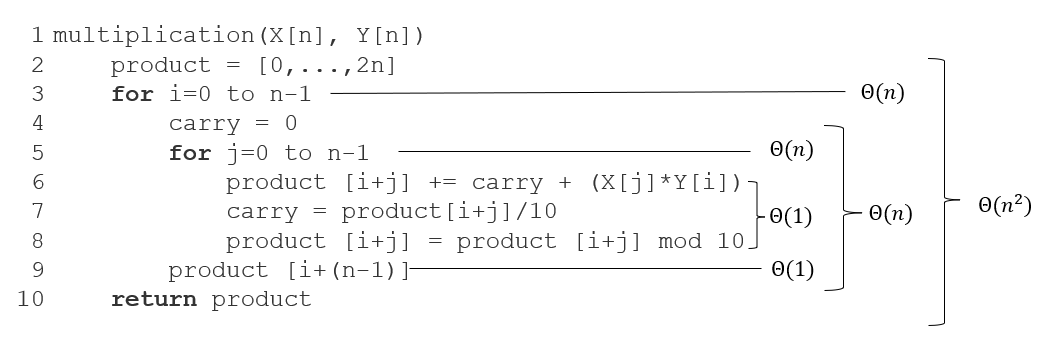
\includegraphics[height=5cm]{imagenes/A1.png}
        \caption{Funci\'on iterativa de la multiplicaci\'on usual}
        \label{fig:my_label}
    \end{figure}
    
    \subsection{Comprobar que \texorpdfstring{$T(n)\in\Theta(n^{2})$}{Lg} donde \texorpdfstring{$T(n)$}{Lg} es la ecuaci\'on de recursividad:}
    $$T(n)=4T(\frac{n}{2})+\Theta(n)$$
    \textbf{Sol.}\\
    Sea $a=4$, $b=2$ y $f(n)=\Theta(n)=Cn$ donde $a\geq1$ y $b>1$ se tiene que
    $$n^{\log_b{a}}=n^{\log_2{4}}=n^{2}$$
    por otro lado se tiene que
    $$f(n)=Cn\in\mathcal{O}(n^{\log_2{4}-\epsilon})=\mathcal{O}(n^{2-1})$$
    Entonces por el Teorema Maestro, caso I)
    $$T(n)=\Theta(n^{\log_b{a}})=\Theta(n^{2})$$
    
    \subsection{Comprobar que \texorpdfstring{$T(n)\in\Theta(n^{\log_2{3}})$}{Lg} donde \texorpdfstring{$T(n)$}{Lg} es la ecuaci\'on de recursividad:}
    $$T(n)=3T(\frac{n}{2})+\Theta(n)$$
    \textbf{Sol.}\\
    Sea $a=3$, $b=2$ y $f(n)=\Theta(n)=Cn$ donde $a\geq1$ y $b>1$ se tiene que
    $$n^{\log_b{a}}=n^{\log_2{3}}$$
    por otro lado se tiene que
    $$f(n)=Cn\in\mathcal{O}(n^{\log_2{3}-\epsilon})$$
    Entonces por el Teorema Maestro, caso I)
    $$T(n)=\Theta(n^{\log_b{a}})=\Theta(n^{\log_2{3}})$$
    
    \subsection{An\'alisis a Priori de la implementaci\'on del algoritmo Kadane para encontrar el máximo subarreglo}%Denzel le pertenece a Erika Giselle Gonzalez Mora y lo ama mucho <3 p.d. pongale 10 profe %
    \textbf{Sol.}\\
    Para la implementaci\'on del algoritmo Kadane tiene como datos de entrada un arreglo A[] de tama\~no $n$ esto para almacenar los elementos con los que interactuara el algoritmo, posterior a eso se declaran 4 variables MaxSum que es la valor m\'aximo global de A[], AcomSum que es un valor m\'aximo local de A[], inicio que guarda el valor del \'indice de inicio del subarreglo  y final que guarda el valor del \'indice del fin del subarreglo.\\
    \\
    As\'i para cada bloque de sentencia del algoritmo se muestra el orden de complejidad para el peor y mejor caso por medio del an\'alisis de segmentos de c\'odigo, v\'ease Figura 8, donde se muestra que $T(n)\in\Theta(n)$.\\
    \begin{figure}[h]
        \centering
        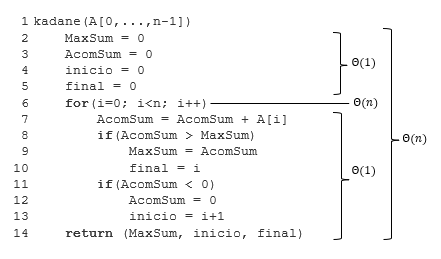
\includegraphics[height=7.0cm]{imagenes/A2.png}
        \caption{Algoritmo Kadane}
        \label{fig:my_label}
    \end{figure}
    \\
    \section{Bibliograf\'ia}
    Brassard, G. (1997). \textit {Fundamentos de Algoritmia}. España: Ed. Prentice Hall.\\[0.4cm]
    Cormen, E. A. (2022). \textit{Introduction To Algorithms}, 3Rd Ed. Phi.\\[0.4cm]
    S\'anchez, P. J. I. (2006). \textit{Análisis y diseño de algoritmos: un enfoque teórico y práctico}. Servicio de Publicaciones y Divulgación Científica de la UMA.
\end{document}